%! TEX program = xelatex
\documentclass{article}
\usepackage{lineno}
\usepackage{amsmath,amssymb,amsthm}
\usepackage{xspace}
\usepackage{microtype}
\usepackage[margin=3cm]{geometry}
\usepackage[]{todonotes}		
\usepackage{mathtools}
\mathtoolsset{showonlyrefs}   
\usepackage{minted} 
	% requires pygments, e.g. pip install pygments. 
	% If you do not install pygments globally on system python, 
	% then you might need to add pygmentize to $PATH, 
	% e.g. in .zprofile (because this is not an interactive shell), add
	%
	%	export PATH=$PATH:$(which pygmentize)
	%
\setminted[scala]{breaklines=true,linenos}
\usepackage{microtype}
 
\usepackage[hyphens]{url}
\usepackage[colorlinks = true,
			citecolor = blue,
			linkcolor = blue]{hyperref}
\usepackage{fontspec}
\setmonofont[Scale=0.9]{Victor Mono}



% inline scala: \mintinline{scala}$val x: => T$
% multiline scala: \begin{minted}{scala}
% scala.collection.IterableOnceOps.max
% \end{minted}



\begin{document}
\title{Programming Assignment: Replicated Key-Value Store \\ \small \href{https://www.coursera.org/learn/scala-akka-reactive/programming/dt8Ku/replicated-key-value-store-audit-track}{audit track} | \href{https://www.coursera.org/learn/scala-akka-reactive/programming/cVXJU/replicated-key-value-store-verified-track}{verified track} }
\author{   From the Coursera course `\href{https://www.coursera.org/learn/scala-akka-reactive/home/welcome}{Programming Reactive Systems}' \\ taught by Roland Kuhn, Konrad Malawski, Martin Odersky, and Julien Richard-Foy.\footnote{Typeset by Calvin Khor}  }

\date{Last compiled: \today}
\maketitle
\tableofcontents
\newpage 
\textbf{NOTE:} This assignment is two weeks long, there will  be no new assignment next week. We recommend not rushing this exercise  and solving it in several steps as you see fit.

To get started,
download the \href{https://moocs.scala-lang.org/~dockermoocs/handouts/scala-3/kvstore.zip}{\texttt{kvstore.zip}}
handout archive file and extract it somewhere on your machine.

\section{Introduction}\label{s:intro}
A key-value store is a very simple form of a database. Its entries are key-value pairs, the key part acting as a unique identifier, and the value being arbitrary data. In recent years, distributed versions of key-value stores have become very popular. Your task in this assignment is to implement a distributed, replicated storage of key-value pairs. Each node (the replicas) in this distributed system will be represented by one actor. You will also have to define some helper actors.

In the simplified version that we will examine, your system will include a primary node (the primary replica), which will be responsible for replicating all changes to a set of secondary nodes (the secondary replicas). The primary and the secondary replica nodes will form a distributed database, where potential replica nodes might join and leave at arbitrary times.

The primary replica will be the only one accepting modification events (insertions and removals) and replicate its current state to the secondaries. Both the primary and the secondary replicas will accept lookup (read) events, although the secondary nodes will be allowed to give results that are ``out-of-date'' since it takes time for the replicas to keep up with the changes on the primary replica.

Compared to a full real-world solution several restricting assumptions are made about the system to make the problem easier to solve:

\begin{itemize}
  \item Updates are only possible on a dedicated node, the primary replica.
  \item The primary (leader) node does not fail during the uptime of the system.
  \item Membership is handled reliably by a provided subsystem (see section ``\hyperref[s:arbiter]{The Arbiter}'').
  \item The update rate is low, meaning that no incoming requests need to be rejected due to system overload.
  \item In case of rejecting an update  the store is left in a possibly inconsistent state which may require a subsequent succeeding write to the same key to repair it.
  \item Clients are expected to not reuse request IDs before the request has been fully processed and responded to.
\end{itemize}

For a more detailed discussion of these restrictions and on how lifting them would affect the solution please refer to the \hyperref[ss:theeffectoftherestrictions]{last section} below.

\textbf{This is a complex assignment. Please read the whole description before attempting to solve the exercise.} In the last section you will find a step-by-step list of which subtasks you need to solve in order to have a complete solution. If you are unable to arrive at a full solution due to time constraints, don’t despair, for you will have learnt a lot along the way.

\section{Overview of the system components}\label{s:overview}

The key-value store and its environment consists of the following components:
\begin{itemize}
  \item \textbf{The clustered key-value store:} A set of nodes that store key value pairs in a distributed fashion, cooperating to maintain a certain set of guarantees (specified in section ``\hyperref[s:systembehavior]{System Behavior - Consistency guarantees}''). This cluster of nodes consists of replicas and the provided Arbiter and \mintinline{scala}!Persistence! modules:

  \item \textbf{Clients:} Entities that communicate with one of the replicas to update or read key-value pairs.
\end{itemize}
You are encouraged to use additional actors in your solution as you see fit.

\subsection{Clients and The KV Protocol}\label{ss:clientsandkv}

Clients are external entities contacting the replica set (your cluster) for reading and writing key-value pairs. It is your responsibility to maintain the consistency guarantees for clients that are described in the next section. Each node participating in the key-value store (primary and secondaries) provides an interface for clients. This interface is a set of messages and corresponding answers that together form the KV Protocol.

The KV Protocol itself contains two subsets of operations:
\begin{enumerate}
  \item Update operations (insertion and removal).
  \item Lookup operation.
\end{enumerate}
Clients contacting the primary node directly can use all operations on the key-value store, while clients contacting the secondaries can only use lookups. The two sets of operations in detail are:
\subsubsection{Update Commands}
\begin{itemize}
  \item \mintinline{scala}{Insert(key, value, id)} - This message instructs the primary to insert the \mintinline{scala}{(key, value)} pair into the storage and replicate it to the secondaries: \mintinline{scala}{id} is a client-chosen unique identifier for this request.
  \item \mintinline{scala}{Remove(key, id)} - This message instructs the primary to remove the key (and its corresponding value) from the storage and then remove it from the secondaries. 
  \item 	A successful \mintinline{scala}{Insert} or \mintinline{scala}{Remove} results in a reply to the client (precisely: to the sender of the update command) in the form of an \mintinline{scala}{OperationAck(id)} message where the \mintinline{scala}{id} field matches the corresponding \mintinline{scala}{id} field of the operation that has been acknowledged.
  \item A failed \mintinline{scala}{Insert} or \mintinline{scala}{Remove} command results in an \mintinline{scala}{OperationFailed(id)} reply. A failure is defined as the inability to confirm the operation within 1 second. See the sections on replication and persistence below for more details.
\end{itemize} 
 \subsubsection{Lookup} 
 \begin{itemize} 
	 \item \mintinline{scala}{Get(key, id)} - Instructs the replica to look up the ``current''' (what current means is described in detail in the next section) value assigned with the key in the storage and reply with the stored value. 
	 \item 	 A \mintinline{scala}{Get} operation results in a \mintinline{scala}{GetResult(key, valueOption, id)} message to be sent back to the sender of the lookup request where the \mintinline{scala}{id} field matches the value in the \mintinline{scala}{id} field of the corresponding \mintinline{scala}{Get} message. The \mintinline{scala}{valueOption} field should contain \mintinline{scala}{None} if the key is not present in the replica or \mintinline{scala}{Some(value)} if a value is currently assigned to the given key in that replica. 
\end{itemize}
 \textbf{All replies sent by the \mintinline{scala}!Replica! shall have that \mintinline{scala}!Replica! as their sender.} 
\section{System Behavior - Consistency guarantees}\label{s:systembehavior}
Let's assume the scenario that one client issues the following commands to the primary replica (starting from empty storage), \textbf{waiting for successful acknowledgement of each operation before proceeding with the next} (see further below for the case of not awaiting confirmation): 
\begin{minted}{scala}
Insert("key1", "a") 
Insert("key2", "1") 
Insert("key1", "b") 
Insert("key2", "2") 
\end{minted}
\subsection{Ordering guarantees for clients contacting the primary replica}\label{ss:orderingguaranteesprimary}
A second client reading directly from the primary is not allowed to see: \begin{itemize} 
\item key1 containing b and then containing a (since a was written before b for key1) 
\item key2 containing 2 and then containing 1 (since 1 was written before 2 for key2) 
\end{itemize} 
In other words, this second client sees the updates in order (although it might miss some updates, so it might see the value 2 for key2 immediately without seeing the intermediate value 1).

In contrast, the second client may observe
\begin{itemize}
    \item key1 containing b and then key2 containing 1
    \item key2 containing 2 and then key1 containing a
\end{itemize}

This means that the ordering guarantee only applies between reads and write to the same key, not across keys. The store may choose to provide stronger semantics to respect ordering across different keys, but clients will not be able to rely on this; the reason is that lifting the restriction of having only one non-failing primary replica would require breaking these stronger guarantees.

\subsection{Ordering guarantees for clients contacting a secondary replica}

For a second client reading from one of the secondary replicas (during a conversation, the replica does not change) the exact same requirements apply as if that client was reading from the primary, with the following addition:

it must be guaranteed that a client reading from a secondary replica will eventually see the following (at some point in the future):

\begin{itemize}
    \item key1 containing b
    \item key2 containing 2
\end{itemize}

\subsection{Ordering guarantees for clients contacting different replicas}

If a second client asks different replicas for the same key, it may observe different values during the time window when an update is disseminated. The client asking for key1 might see

\begin{itemize}
    \item answer b from one replica
    \item and subsequently answer a from a different replica
\end{itemize}

As per the rule stated in the previous section, and assuming that the client keeps asking repeatedly, eventually all reads will result in the value b if no other updates are done on key1.

Eventual consistency means that given enough time, all replicas settle on the same view. This also means that when you design your system \textbf{clients contacting multiple replicas at the same time are not required to see any particular ordering.} You do not need to design your solution for such scenarios and the grading system will not test these either.

\subsection{Durability guarantees of updates for clients contacting the primary replica}

The previous two sections prescribed possible transitions that the clients are allowed to experience on key updates. In this section, we will see what guarantees acknowledgement messages must obey (on the primary replica).

Whenever the primary replica receives an update operation (either Insert or Remove) it must reply with an \mintinline{scala}!OperationAck(id)! or \mintinline{scala}!OperationFailed(id)! message, to be sent at most 1 second after the update command was processed (the \mintinline{scala}!ActorSystem!’s \mintinline{scala}!timer! resolution is deemed to be sufficiently precise for this).

A positive \mintinline{scala}!OperationAck! reply must be sent as soon as

\begin{enumerate}
	\item the change in question has been handed down to the \mintinline{scala}!Persistence! module (provided) \textbf{and} a corresponding acknowledgement has been received from it (the persistence module is ``flaky''—it fails randomly from time to time—and it is your task to keep it alive while retrying unacknowledged persistence operations until they succeed, see the \hyperref[ss:persistence]{persistence} section for details)
	\item replication of the change in question has been initiated \textbf{and} all of the secondary replicas have acknowledged the replication of the update.
\end{enumerate}

If replicas leave the cluster, which is signalled by sending a new \mintinline{scala}!Replica! message to the primary, then outstanding acknowledgements of these replicas must be waived. This can lead to the generation of an \mintinline{scala}!OperationAck! triggered indirectly by the Replicas message.

A negative \mintinline{scala}!OperationFailed! reply must be sent if the conditions for sending an \mintinline{scala}!OperationAck! are not met within the 1 second maximum response time.

\subsection{Consistency in the case of failed replication or persistence}

Assuming in the above scenario that the last write fails (i.e. an \mintinline{scala}!OperationFailed! is returned), replication to some replicas may have been successful while it failed on others. Therefore in this case the property that eventually all replicas converge on the same value for key2 is not provided by this simplified key–value store. In order to restore consistency a later write to key2 would have to succeed.

One consequence of this restriction is that each replica uses this  freedom to immediately hand out the updated value to subsequently  reading clients, even before the the new value has been persisted locally, and no rollback is attempted in case of failure.

\subsection{Which value to expect while an update is outstanding?}

Sending an update request for a key followed by a \mintinline{scala}!Get! request for the same key without waiting for the acknowledgement of the update is allowed to return either the old or the new value (or a third value if another client concurrently updates the same key). An example, assuming only this one client at this time:

\begin{minted}{scala}
Insert("key1", "a")
// <await confirmation> 
Insert("key1", "b") Get("key1") 
\end{minted}

The replies for the last two requests may arrive in any order, and the reply for the \mintinline{scala}!Get! request may either contain \mintinline{scala}!"a"! or \mintinline{scala}|"b"|.

\section{The Arbiter}\label{s:arbiter}

The Arbiter is an external subsystem that will be provided for use. The Arbiter follows a simple protocol:

\begin{itemize}
    \item New replicas must first send a \mintinline{scala}!Join! message to the Arbiter signaling that they are ready to be used.
    \item The \mintinline{scala}!Join! message will be answered by either a \mintinline{scala}!JoinedPrimary! or \mintinline{scala}!JoinedSecondary! message indicating the role of the new node; the answer will be sent to the sender of the \mintinline{scala}!Join! message. The first node to join will get the primary role, other subsequent nodes are assigned the secondary role.
    \item The arbiter will send a \mintinline{scala}!Replicas! message to the primary replica whenever it receives the \mintinline{scala}!Join! message; for this reason the sender of the \mintinline{scala}!Join! message must be the replica Actor itself. This message contains the set of available replica nodes including the primary and all the secondaries.
\end{itemize}

All messages sent by the Arbiter will have the Arbiter as their sender.

\section{The Replicas}\label{s:replicas}

You have to provide an Actor representing a node of the system. Its declaration is:

\begin{minted}{scala}
class Replica(val arbiter: ActorRef) extends Actor 
\end{minted}

Please note that in this exercise the nodes (i.e. actors) are executed within the same JVM, but the problems and their solutions apply equally when distributing the system across multiple network hosts.

When your actor starts, it must send a \mintinline{scala}!Join! message to the Arbiter and then choose between primary or secondary behavior according to the reply of the Arbiter to the \mintinline{scala}!Join! message (a \mintinline{scala}!JoinedPrimary! or \mintinline{scala}!JoinedSecondary! message).

The primary replica must provide the following features:

\begin{itemize}
    \item The primary must accept update and lookup operations from clients following the Key-Value protocol like \mintinline{scala}{Insert}, \mintinline{scala}{Remove} or \mintinline{scala}{Get}s as it is described in the “\hyperref[ss:clientsandkv]{Clients and The KV Protocol}” section, respecting the consistency guarantees described in “\hyperref[ss:orderingguaranteesprimary]{Guarantees for clients contacting the primary replica}”.
    \item The primary must replicate changes to the secondary replicas of the system. It must also react to changes in membership (whenever it gets a Replicas message from the Arbiter) and start replicating to newly joined nodes, and stop replication to nodes that have left; the latter implies terminating the corresponding \mintinline{scala}!Replicator! actor. More details can be found in the section ``\hyperref[ss:replicationprotocol]{Replication Protocol}''.
\end{itemize}

The secondary replicas must provide the following features:

\begin{itemize}
    \item The secondary nodes must accept the lookup operation (\mintinline{scala}{Get}) from clients following the Key-Value protocol while respecting the guarantees described in “Guarantees for clients contacting the secondary replica”.
    \item The replica nodes must accept replication events, updating their current state (see “\hyperref[ss:replicationprotocol]{Replication Protocol}”).
\end{itemize}

\subsection{The Replication Protocol}\label{ss:replicationprotocol}

Apart from providing the KV protocol for external clients, you must implement another protocol involving the primary and secondary replicas and some newly introduced helper nodes. The KV store will use this protocol to synchronize its state between nodes.

When a new replica joins the system, the primary receives a new \mintinline{scala}!Replicas! message and must allocate a new actor of type \mintinline{scala}!Replicator! for the new replica; when a replica leaves the system its corresponding \mintinline{scala}!Replicator! must be terminated. The role of this \mintinline{scala}!Replicator! actor is to accept \textbf{update events}, and propagate the changes to its corresponding replica (i.e. there is exactly one \mintinline{scala}!Replicator! per secondary replica). \textbf{Also, notice that at creation time of the \mintinline{scala}!Replicator!, the primary must forward update events for every key-value pair it currently holds to this \mintinline{scala}!Replicator!.}

Your task for this protocol will be to provide an \mintinline{scala}!Actor! representing a \mintinline{scala}!Replicator!. Its declaration is:

\begin{minted}{scala}
class Replicator(val replica: ActorRef) extends Actor 
\end{minted}

The protocol includes two pairs of messages. The first one is used by the replica actor which requests replication of an update:

\begin{itemize}
    \item \mintinline{scala}{Replicate(key, valueOption, id)} is sent to the \mintinline{scala}!Replicator! to initiate the replication of the given update to the key; in case of an Insert operation the \mintinline{scala}{valueOption} will be \mintinline{scala}{Some(value)} while in case of a Remove operation it will be \mintinline{scala}{None}. The sender of the Replicate message shall be the \mintinline{scala}!Replica! itself.
    \item \mintinline{scala}{Replicated(key, id)} is sent as a reply to the corresponding Replicate message once replication of that update has been successfully completed (see \mintinline{scala}!SnapshotAck!). The sender of the \mintinline{scala}!Replicated! message shall be the \mintinline{scala}!Replicator!.
\end{itemize}
The second pair is used by the replicator when communicating with its partner replica:
\begin{itemize}
    \item \mintinline{scala}{Snapshot(key, valueOption, seq)} is sent by the \mintinline{scala}!Replicator! to the appropriate secondary replica to indicate a new state of the given key. \mintinline{scala}{valueOption} has the same meaning as for \mintinline{scala}!Replicate! messages. The sender of the \mintinline{scala}!Snapshot! message shall be the \mintinline{scala}!Replicator!. The \mintinline{scala}!Snapshot! message provides a sequence number (\mintinline{scala}{seq}) to enforce ordering between the updates. Updates for a given secondary replica must be processed in contiguous ascending sequence number order; this ensures that updates for every single key are applied in the correct order. Each \mintinline{scala}!Replicator! uses its own number sequence starting at zero. When a snapshot arrives at a \mintinline{scala}!Replica! with a sequence number which is greater than the currently expected number, then that snapshot must be ignored (meaning no state change and no reaction). When a snapshot arrives at a \mintinline{scala}!Replica! with a sequence number which is smaller than the currently expected number, then that snapshot must be ignored and immediately acknowledged as described below. The sender reference when sending the Snapshot message must be the \mintinline{scala}!Replicator! actor (not the primary replica actor or any other).
    \item \mintinline{scala}{SnapshotAck(key, seq)} is the reply sent by the secondary replica to the \mintinline{scala}!Replicator! as soon as the update is persisted locally by the secondary replica. The replica might never send this reply in case it is unable to persist the update. The sender of the \mintinline{scala}!SnapshotAck! message shall be the secondary \mintinline{scala}!Replica!. The acknowledgement is sent immediately for requests whose sequence number is less than the next expected number. The expected number is set to the greater of the previously expected number and the sequence number just acknowledged, incremented by one
\end{itemize}

You should note that the \mintinline{scala}!Replicator! may handle multiple snapshots of a given key in parallel (i.e. their replication has been initiated but not yet completed). It is allowed—but not required—to batch changes before sending them to the secondary replica, provided that each replication request is acknowledged properly and in the right sequence when complete. An example:

\begin{minted}{scala}
Replicate("a_key", Some("value1"), id1) 
Replicate("a_key", Some("value2"), id2) 
\end{minted}
might have reached the \mintinline{scala}!Replicator! before it got around to send a \mintinline{scala}!Snapshot! message for \mintinline{scala}!"a_key"! to its replica. These two messages could then result in only the following replication message

\begin{minted}{scala}
Snapshot("a_key", Some("value2"), seq) 
\end{minted}

skipping the state where \mintinline{scala}!"a_key"! contains the value \mintinline{scala}!"value1"!.

Since the replication protocol is meant to symbolize remote replication you must consider the case that either a Snapshot message or its corresponding \mintinline{scala}!SnapshotAck! message is lost on the way. Therefore the \mintinline{scala}!Replicator!  must make sure to periodically retransmit all unacknowledged changes.  For grading purposes it is assumed that this happens roughly every 100  milliseconds. To allow for batching (see above) we will assume that a  lost \mintinline{scala}!Snapshot! message will lead to a resend at most 200 milliseconds after the \mintinline{scala}!Replicate! request was received (again, the \mintinline{scala}!ActorSystem!’s \mintinline{scala}!scheduler! service is considered precise enough for this purpose).

\subsection{Persistence}\label{ss:persistence}

Each replica will have to submit incoming updates to the local \mintinline{scala}!Persistence! actor and wait for its acknowledgement before confirming the update to the requester. In case of the primary, the requester is a client which sent an \mintinline{scala}!Insert! or \mintinline{scala}!Remove! request and the confirmation is an \mintinline{scala}!OperationAck!, whereas in the case of a secondary the requester is a \mintinline{scala}!Replicator! sending a \mintinline{scala}!Snapshot! and expecting a \mintinline{scala}!SnapshotAck! back.

The used message types are:

\begin{itemize}
    \item \mintinline{scala}{Persist(key, valueOption, id)} is sent to the \mintinline{scala}!Persistence! actor to request the given state to be persisted (with the same field description as for the Replicate message above).
    \item \mintinline{scala}{Persisted(key, id)} is sent by the \mintinline{scala}!Persistence! actor as reply in case the corresponding request was successful; no reply is sent otherwise. The reply is sent to the sender of the Persist message. Note, however, that the sender of the \mintinline{scala}!Persisted! message might not be the \mintinline{scala}!Persistence! actor (in some tests, the \mintinline{scala}!Persisted! message will be sent by a wrapper actor).
\end{itemize}

The provided implementation of this persistence service is a mock in the true sense, since it is rather unreliable: every now and then it will fail with an exception and not acknowledge the current request. It is the job of the \mintinline{scala}!Replica! actor to create and appropriately supervise the \mintinline{scala}!Persistence! actor; for the purpose of this exercise any strategy will work, which means that you can experiment with different designs based on resuming, restarting or stopping and recreating the \mintinline{scala}!Persistence! actor. To this end your \mintinline{scala}!Replica! does not receive an \mintinline{scala}!ActorRef! but a \mintinline{scala}!Props! for this actor, implying that the \mintinline{scala}!Replica! has to initially create it as well.

For grading purposes it is expected that \mintinline{scala}!Persist! is retried before the 1 second response timeout in case persistence failed. The \mintinline{scala}!id! used in retried \mintinline{scala}!Persist! messages must match the one which was used in the first request for this particular update.

\section{Your Task}\label{s:yourtask}

Since this assignment is a longer one, we have prepared the test suite in a way that supports the solution step by step. In the following you can find a suggestion for how to proceed with the solution, but you can of course choose any path leading up to twenty points that you like.

\begin{enumerate}
    \item Implement the primary replica role so that it correctly responds to the KV protocol messages without considering persistence or replication.
    \item Implement the secondary replica role so that it correctly responds to the read-only part of the KV protocol and accepts the replication protocol, without considering persistence.
    \item Implement the replicator so that it correctly mediates between replication requests, snapshots and acknowledgements.
    \item Implement the use of persistence at the secondary replicas.
    \item Implement the use of persistence and replication at the primary replica.
    \item Implement the sending of the initial state replication to newly joined replicas.
\end{enumerate}

\subsection{Hints, Tips}

The logic for collecting acknowledgements of persistence and replication can be made such that it is usable both in primary and secondary replicas.

You should write (versions of) tests which exercise the behavior under unreliable persistence (i.e. when using a \mintinline{scala}!Persistence! actor created with \mintinline{scala}!flaky = true!) or unreliable communication between primary and secondaries. The latter can be done by having the Arbiter wrap the secondary nodes’ \mintinline{scala}!ActorRef!s in small actors which normally  forward messages but sometimes forget to do so. The grading process  involves such a test suite as well.

Resending snapshots from the \mintinline{scala}!Replicator! without  pause is not the intended solution—the resend rate needs to be kept  reasonable. This fact is exploited implicitly by the test suite in step  3.

\subsection{The Effect of the Restrictions}\label{ss:theeffectoftherestrictions}
This section is meant to offer further insights for those who want to  take the assignment as a starting point for continuing their own  studies beyond what the course provides. It is not necessary to read  this section in order to complete the assignment.

\subsubsection{Updates are only accepted by a distinguished primary replica}

Accepting writes only on one node at any given time simplifies  conflict resolution, because request arrival order at that node can be  used to serialize updates to a given key. The downside of this is that  this node clearly limits the amount of requests that can be handled per second, it is a single point of bottleneck.

In order to scale the possible update rate beyond what a single node  can digest it would also be possible to divide the key space into shards  and distribute them across the members, making each member a primary  for a certain portion of the key space. The clients would then need to  either be told which one the right node is for updating a certain key,  or every node could include a ConsistentHashingRouter which dispatches  incoming requests to the right node on the client’s behalf (see the  diagram below). Moving the primary role for a shard from one member to  another would then be necessary to rebalance the allocation when nodes  join or leave the cluster.

The service which determines the placement of shards does not need to be a single point of bottleneck,  as we can see the distribution of shards by using consistent hashing  can be done without going through a central point. The only thing that  needs special care is the hand-off period when shards move between  nodes.
\begin{center}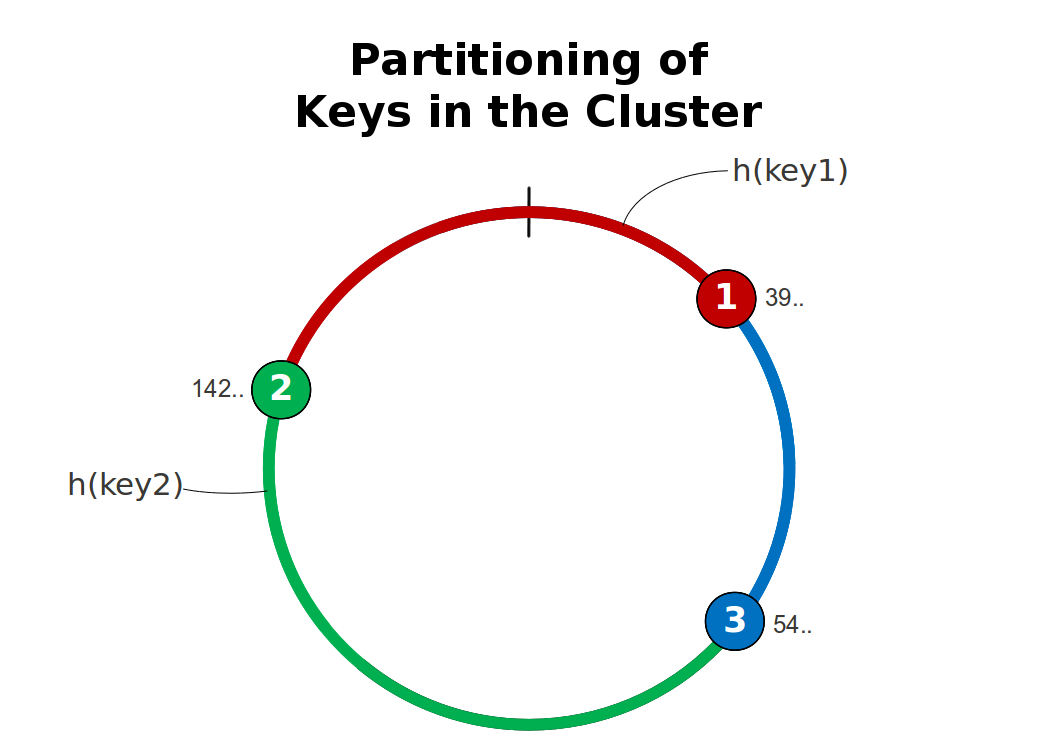
\includegraphics[scale=0.4]{partitioningofkeysinthecluster.png}
\end{center}	


\subsubsection{The primary node does not fail}

A real system would have to tolerate a failure of the primary node,  which otherwise would be a single point of failure, making the system  not resilient. In order to support this, the primary role must be  transferred by the arbiter to another node, which transitions from  secondary to primary and starts accepting updates. During this transition  updates will be left without a reply, but since confirmations are only  sent out after all replicas have acknowledged an update, the new primary  node will be able to continue where the old one left off.

One problem are unconfirmed or even rejected updates which have in  fact been accepted by all secondary replicas. The store will in this  case be internally consistent, but its contents possibly does not match  what the client assumes if it received an \mintinline{scala}!OperationFailed!  message. Having received that message signals a possibly inconsistent  state due to other reasons as well, and it could be an option to require  the client to attempt to repair it by sending another write to the same  key if needed.

\subsubsection{Membership is handled reliably by a provided subsystem}

A service which reliably handles membership is available in the form  of the Akka Cluster module. The arbiter of this assignment can be a 
\href{http://doc.akka.io/docs/akka/2.2.3/scala/cluster-usage.html#Cluster_Singleton_Pattern}{ClusterSingleton}
  to which replicas register and which uses \mintinline{scala}!DeathWatch! to monitor them,  or the cluster membership list could be used directly, determining the  primary role by sorting the member addresses and using the first one.

  \subsubsection{The update rate is low}

Without this restriction the resend mechanism for example in the \mintinline{scala}!Replicator! would have to manage the size of the buffer in which snapshots are kept while awaiting their acknowledgement. This means that the replication mechanism could either lose updates or the \mintinline{scala}!Replica! would need to start rejecting requests with \mintinline{scala}!OperationFailed! as soon as a limit on the number of outstanding requests is exceeded.

Especially when considering the next restriction, latency of confirmations is a performance sensitive  topic. One further possible optimization is to distribute the burden of  ensuring consistency between the primary and secondary nodes by  requiring that only a certain number of secondaries have sent their  confirmation before ack	nowledging an update. In order to restore  consistency in case of a replication failure (e.g. if the primary stops  working for whatever reason) the secondaries have to ask their peers for  the key and a reply is only sent once enough have replied with the same  value. If the number of write confirmations is $W$ and the count of  agreeing reads is denoted $R$, then the condition for consistency is  $R+W>N$, where $N$ is the total number of replicas. This equation must be  interpreted with some care because $N$ can change during a replication or read process.

\subsubsection{Disregarding inconsistencies after OperationFailed}

This is the toughest restriction to lift because it touches on the  fundamental choice of which flavor of weak consistency eventually shall  be reached. The restriction allows the system to stay responsive in case  of failure (by providing an \mintinline{scala}!OperationFailed! reply), but making that reply mean that the update will eventually disappear from all nodes is not possible in general.

Assuming that the primary does not fail for a sufficiently long time  period after the operation failure, the first step would be to ensure  that for a given key only up to one update can be “in flight”  at any given time. If the primary determines that this update has  failed, it will then replicate the previous state for that key to all  replicas, awaiting confirmation without a timeout. This favors  consistency over availability, since it makes the service of updating that key unavailable while the system is experiencing a malfunction.

\subsubsection{Clients are expected not to reuse request IDs}

This restriction makes your solution simpler and it also removes the  need for some grading tests which would have been hard to formulate in a  way which does not assume too much about your solution. In a real system you might even find this restriction as specified operational requirement.
\end{document}

